%
% main.tex -- Paper zum Thema <rossby>
%
% (c) 2020 Autor, OST Ostschweizer Fachhochschule
%
% !TEX root = papers/rossby/papers/rossby/buch.tex
% !TEX encoding = UTF-8
% !TeX spellcheck = de-CH

\chapter{Rossby Wellen\label{chapter:rossby}}
\kopflinks{Rossby Wellen}
\begin{refsection}
	\chapterauthor{Michael Schmid}

    \section{Einleitung}
    \section{Einleitung} \label{poinbendix:section:einleitung}

Der Satz von Poincaré-Bendixson beschreibt mögliche Bahnkurven von zweidimensionalen dynamischen Systemen.
Unter einem dynamischen System versteht man die Bewegung durch ein Vektorfeld entlang der Vektoren.

Beschrieben wird dies durch ein Differentialgleichungssystem in den Koordinaten $x$ und $y$ der Form
\begin{equation*}
\frac{d}{dt}
\begin{pmatrix}x\\y\end{pmatrix}
=
f(x,y),
\end{equation*}
wobei $f(x,y)$ eine vektorwertige Funktion darstellt.
Im ganzen Kapitel wird immer implizit von Differentialgleichungssystemen dieser Art gesprochen.
Geschrieben werden sie aber in den Beispielen immer als zwei Differentialgleichungen
\begin{align*}
    \dot{x} &= f_x(x, y) \\
    \dot{y} &= f_y(x, y).
\end{align*}

Unabhängig von der Natur des zweidimensionalen dynamischen Systems schränkt der Satz von Poincaré-Bendixson die möglichen Bahnkurven auf drei Fälle ein.
Somit können Bahnkurven in zwei Dimensionen kein chaotisches oder unberechenbares Verhalten zeigen.

Im ersten Abschnitt \ref{poinbendix:section:nullklinen} wird ein intuitives Verständnis über das Verhalten solcher Bahnkurven mithilfe der sogenannten Nullklinen aufgebaut.
Dies hilft uns den eigentlichen Satz in \ref{poinbendix:section:poinbendix} besser zu verstehen.
Neben dem Satz von Poincaré-Bendixson finden sich in diesem Abschnitt auch einige Beispiele.

    \section{Grundlagen}
    
\subsection{Idealisiertes zonales und meridionales Windfeld}

In der Meteorologie werden Windgeschwindigkeiten in ein rechtwinkliges Koordinatensystem zerlegt. 
Die {zonal}e Komponente \(u\) beschreibt die Geschwindigkeit in Ost-West-Richtung, 
die {meridional}e Komponente \(v\) jene in Nord-Süd-Richtung. 
Positive Werte von \(u\) stehen für eine Strömung nach Osten, positive Werte von \(v\) für eine Strömung nach Norden.


Abbildung~\ref{fig:zonal_wind} zeigt ein idealisiertes zonales Windfeld, bei
dem ausschliesslich eine Ost-West-Strömung vorliegt (\(v = 0\)). Die
Geschwindigkeit hängt von der geographischen Breite \(\varphi\) ab und folgt der
Beziehung
\begin{equation}
	u = U_0 \cdot \sin^2(\varphi).
	\label{rossby:eq:zonal_wind}
\end{equation}
Ein Druckgradient oder eine vertikale Struktur sind nicht berücksichtigt, es handelt sich um ein rein theoretisches, horizontal homogenes Modell.

\begin{figure}
	\centering
	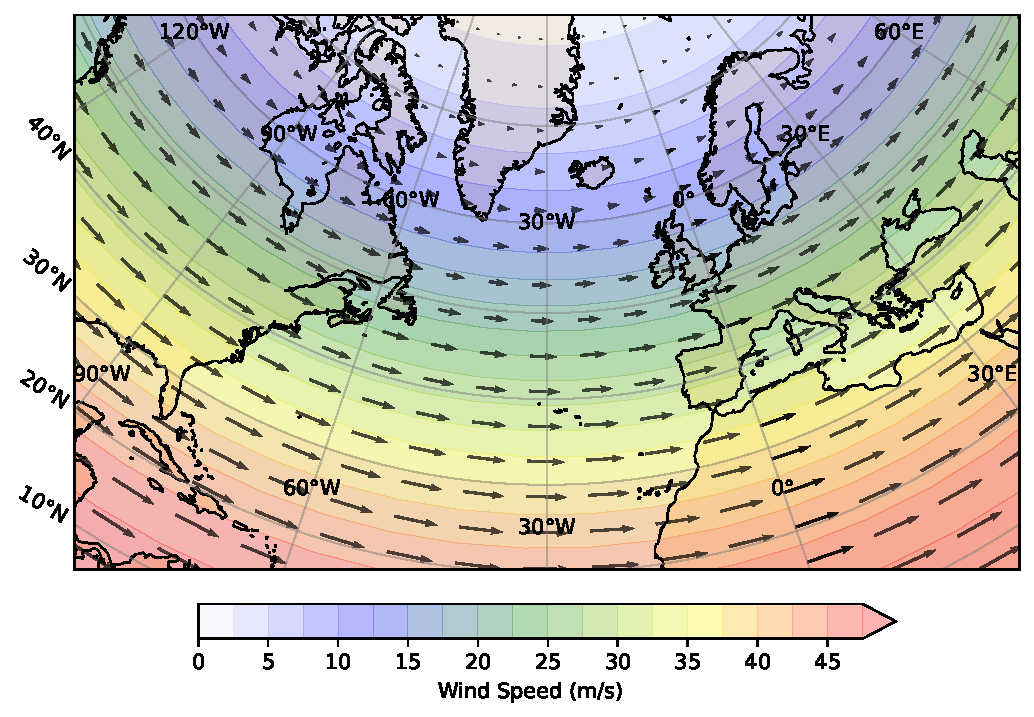
\includegraphics[width=\textwidth, trim=1cm 0cm 2cm 0cm, clip]{papers/rossby/images/zonal_wind_plot.pdf}
	\caption{Idealisiertes zonales Windfeld (\(v=0\)), Geschwindigkeit \(u = U_0 \cdot \sin^2(\varphi)\).}
	\label{fig:zonal_wind}
\end{figure}

\noindent
Abbildung~\ref{fig:meridional_wind} zeigt dagegen ein idealisiertes meridionales Windfeld, bei dem nur eine Nord-Süd-Strömung existiert (\(u = 0\)).
Die Geschwindigkeit hängt hier von der Breite ab nach
\begin{equation}
	v = V_0 \cdot \cos(\varphi).
	\label{rossby:eq:meridional_wind}
\end{equation}
Auch dieses Feld ist frei von Druckgradienten und vertikaler Struktur und dient der isolierten Betrachtung meridionaler Strömungskomponenten.

\begin{figure}
	\centering
	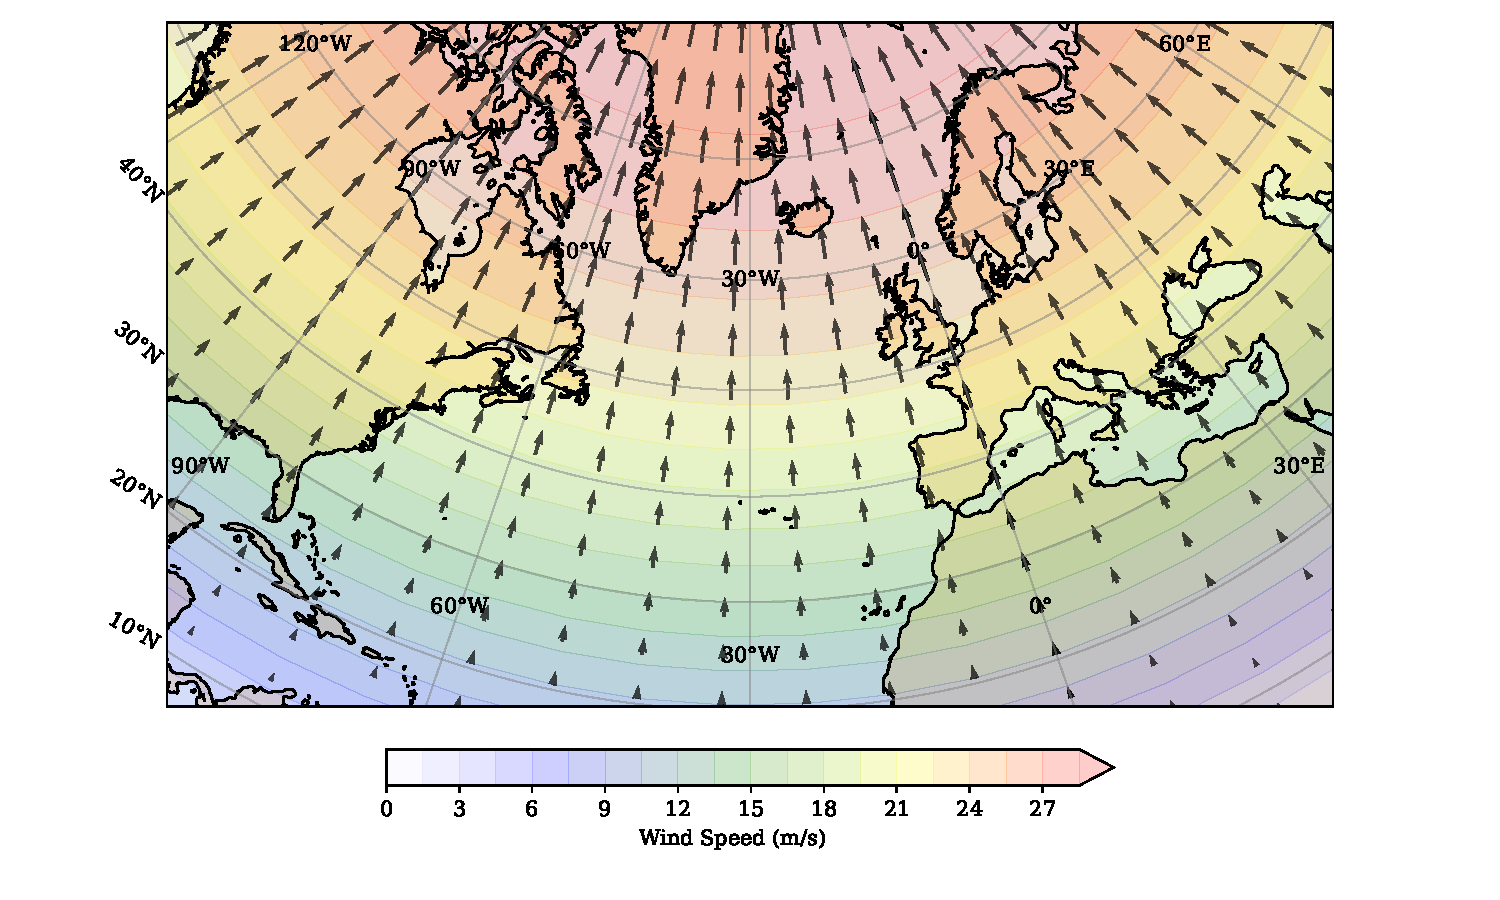
\includegraphics[width=\textwidth, trim=1cm 0cm 2cm 0cm, clip]{papers/rossby/images/meridional_wind_plot.pdf}
	\caption{Idealisiertes meridionales Windfeld (\(u=0\)), Geschwindigkeit \(v = V_0 \cdot \cos(\varphi)\).}
	\label{fig:meridional_wind}
\end{figure}

\subsection{Die Drehung der Erde und die Coriolis-Kraft}

Die Erde rotiert einmal pro Tag um ihre eigene Achse. In einem rotierenden
Bezugssystem wie der Erde treten dabei Scheinkräfte auf, die in der klassischen
Mechanik berücksichtigt werden müssen. Eine davon ist die {Coriolis-Kraft},
welche bewegte Luft- und Wassermassen auf der {Nordhalbkugel} nach rechts und
auf der {Südhalbkugel} nach links ablenkt. Ihre Wirkung ist maximal an den
Polen und verschwindet am Äquator. Die Coriolis-Kraft ist keine reale Kraft,
sondern eine Folge der Drehung des Koordinatensystems.

Wir betrachten ein lokales kartesisches Koordinatensystem auf der Erdoberfläche mit den Achsen
\begin{equation}
(x,y,z) = (\text{Ost–West}, \; \text{Nord–Süd}, \; \text{Vertikal}).
\end{equation}
Dabei bezeichnet \(y\) die Entfernung in Nord–Süd-Richtung (Meridionalrichtung). 
Da die Erde den Radius \(a\) besitzt, ergibt sich für kleine Breitenänderungen \(\mathrm{d}\varphi\) die entsprechende Nord–Süd-Distanz
\begin{equation}
\mathrm{d}y = a \, \mathrm{d}\varphi.
\end{equation}
Durch Integration erhält man
\begin{equation}
y = a \, \varphi \qquad (\varphi ).
\end{equation}

Der Coriolis-Parameter ist definiert als
\begin{equation}
f(\varphi) = 2 \, \Omega \, \sin(\varphi),
\end{equation}
wobei \(\Omega\) die Erdrotationsrate bezeichnet. 
Die Breitenänderung von \(f\) mit der Nord–Süd-Koordinate \(y\) ergibt den \(\beta\)-Parameter:
\begin{equation}
\beta = \frac{\partial f}{\partial y} 
      = \frac{\partial f}{\partial \varphi} \cdot \frac{\partial \varphi}{\partial y}.
\end{equation}
Da gilt
\begin{equation}
\frac{\partial f}{\partial \varphi} = 2 \Omega \cos(\varphi), 
\qquad 
\frac{\partial \varphi}{\partial y} = \frac{1}{a},
\end{equation}
folgt
\begin{equation}
\beta = \frac{2 \Omega \cos(\varphi)}{a}.
\end{equation}

Damit ist klar: \(y\) ist die Nord–Süd-Koordinate auf der Erdoberfläche, 
direkt über \(y = a \varphi\) mit der geographischen Breite verknüpft.


\begin{beispiel}
\paragraph{Rechenbeispiel: Velofahren in Zürich}

Wir berechnen die Coriolis-Kraft auf einen Radfahrer in Zürich.

\begin{description}
	\item[Gegeben:] Geschwindigkeit \(v = 8.33\,\mathrm{m/s}\) (30\,km/h), Masse \(m =
	      80\,\mathrm{kg}\), geographische Breite \(\varphi = 47^\circ\) (Zürich),
	      Erdrotationsrate \(\Omega \approx 7.292 \times 10^{-5}\,\mathrm{rad/s}\).
	\item[Formel:]
	      \[
		      F_C = 2\,m\,v\,\Omega\,\sin(\varphi)
	      \]
	\item[Einsetzen:]
	      \[
		      F_C \approx 2 \cdot 80 \cdot 8.33 \cdot 7.292 \times 10^{-5} \cdot \sin(47^\circ)
		      \approx 0.070\,\mathrm{N}
	      \]
\end{description}

\end{beispiel}
\noindent
Die resultierende Kraft von rund \(0.07\,\mathrm{N}\) ist für uns im Alltag kaum spürbar, prägt jedoch die grossräumige Atmosphärendynamik.
Sie bewirkt, dass Luftmassen nicht direkt vom Hoch- zum Tiefdruckgebiet strömen, sondern entlang der Isobaren gelenkt werden.
Dieser Effekt ist massgeblich für die Westwinddrift in den mittleren Breiten und bildet die physikalische Grundlage für Rossby-Wellen.

\subsection{Die Approximation der \(\beta\)-Ebene }

Die \(\beta\)-Ebene ist eine lokale Approximation der Erdkugel in der Umgebung
einer bestimmten geographischen Breite~\(\varphi_0\)
(Abbildung~\ref{fig:beta_plane}). Ziel dieser Vereinfachung ist es, die
Breitenabhängigkeit der Coriolis-Kraft in mathematischen Modellen handhabbar zu
machen. Der \emph{Coriolis-Parameter} wird dazu in der Nähe der Referenzbreite linear
entwickelt:
\begin{equation}
	f(y) = f_0 + \beta y,
	\label{rossby:eq:beta_plane}
\end{equation}
wobei $f_0 = 2 \Omega \sin(\varphi_0)$ der Coriolis-Parameter an der
Referenzbreite ist und $y$ die meridionale Entfernung vom
Referenzbreitenkreis bezeichnet.
Der Term
\begin{equation}
	f_0 = 2\Omega \sin(\phi_0)
	\label{rossby:eq:coriolis_parameter_ref}
\end{equation}
bezeichnet den Coriolisparameter an der Referenzbreite, und
\begin{equation}
	\beta = \left.\frac{\partial f}{\partial y}\right|_{\phi_0} = \frac{2\Omega \cos(\phi_0)}{a}
	\label{rossby:eq:beta_parameter_ref}
\end{equation}
beschreibt die Änderung von $f$ mit der geographischen Breite; $a$ ist der
Erdradius. Diese Darstellung erlaubt es, lokale Phänomene wie Rossby-Wellen auf
einer idealisierten Ebene zu analysieren, ohne die volle Kugelgeometrie der
Erde berücksichtigen zu müssen.

\begin{figure}
	\centering
	\begin{tikzpicture}[scale=2]
		% Tilted group (Earth and axes)
		\begin{scope}[rotate around={23.5:(0,0)}]
			% Axes
			\draw (-2,0) -- (2,0);
			\draw[->] (0,-2) -- (0,2) node[above] {Pol};

			% Earth (circle)
			\draw[thick] (1,0) arc[start angle=0, end angle=360, radius=1];

			% 3D-style spinning arrow (elliptical path)
			\draw[->, thick] ({0.3*cos(10)},{1.5 + 0.1*sin(10)})
			arc[start angle=10, end angle=320, x radius=0.3, y radius=0.1];

			% Point on the circle
			\fill[red] (30:1) circle[radius=0.05] node[right] {$P$};
			\draw[blue, thick] ($(30:1) + (120:0.5)$) -- ($(30:1) + (-60:0.5)$);

			% Connection from center to P
			\draw[] (0,0) -- (30:1);

			% Angle phi
			\draw[thick] (0.5,0) arc[start angle=0, end angle=30, radius=0.5];
			\node at (0.65,0.12) {$\varphi$};
		\end{scope}
	\end{tikzpicture}
	\caption{Schematische Darstellung der $\beta$-Ebenen-Approximation um einen Referenzbreitenkreis.
		Der rote Punkt \(P\) markiert die Referenzbreite, in deren Umgebung die Erdoberfläche als tangentiale Ebene angenähert wird.
		Die blaue Linie zeigt den Tangentialebene durch \(P\), der Pfeil die Rotationsrichtung der Erde. 
		Der Winkel \(\varphi\) beschreibt die geographische Breite des Punktes \(P\).}
	\label{fig:beta_plane}
\end{figure}

    \section{Vorticity}
    
\subsection{Vorticity – Wirbelstärke in der Atmosphäre}

Die grossräumige Bewegung der Luft in der Atmosphäre lässt sich nicht nur durch die
Geschwindigkeit beschreiben, sondern auch durch ihre Rotationseigenschaften.
Diese Eigenschaft wird durch die sogenannte \emph{Vorticity} (Wirbelstärke)
\index{Vorticity}%
\index{Wirbelstärke}%
quantifiziert. Physikalisch beschreibt sie die Tendenz eines Luftpakets, sich
um seine eigene vertikale Achse zu drehen.

Mathematisch ist die Vorticity definiert als Rotation des
Geschwindigkeitsfeldes:
\begin{equation}
	\vec{\zeta} = \nabla \times \vec{u}.
	\label{rossby:eq:vorticity}
\end{equation}
Für grossräumige Strömungen in der Atmosphäre betrachtet man hauptsächlich die vertikale Komponente dieser Rotation, die sogenannte \emph{relative Vorticity}.
\index{relative Vorticity}%
\index{Vorticity, relativ}%
In kartesischen Koordinaten ergibt sich diese im einfachsten Fall zu:
\begin{equation}
	\zeta = \frac{\partial v}{\partial x} - \frac{\partial u}{\partial y},
	\label{rossby:eq:relative_vorticity}
\end{equation}
wobei \(u\) und \(v\) die zonale bzw. meridionale Windkomponente bezeichnen.
Positive Vorticity (\(\zeta > 0\)) steht für eine zyklonale Rotation (auf der Nordhalbkugel gegen den Uhrzeigersinn), negative Vorticity (\(\zeta < 0\)) für eine antizyklonale Rotation (im Uhrzeigersinn).
\index{zyklonale Rotation}%
\index{antizyklonale Rotation}%
\begin{figure}
	\centering
	% Erste Reihe
	\begin{minipage}{0.32\linewidth}
		\centering
		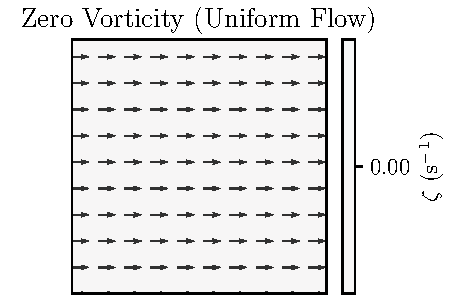
\includegraphics[width=\linewidth]{papers/rossby/images/vorticity_plot0.pdf}\\
		{\small \( \vec{u} = (2,0),\ \zeta = 0\)}
	\end{minipage}
	\begin{minipage}{0.32\linewidth}
		\centering
		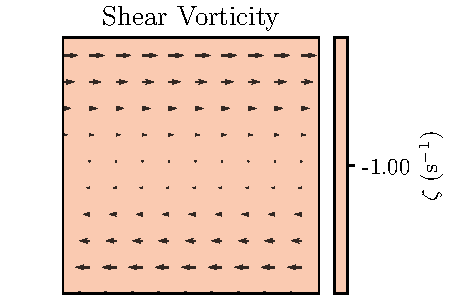
\includegraphics[width=\linewidth]{papers/rossby/images/vorticity_plot1.pdf}\\
		{\small \( \vec{u} = (y,0),\ \zeta = -1\)}
	\end{minipage}
	\begin{minipage}{0.32\linewidth}
		\centering
		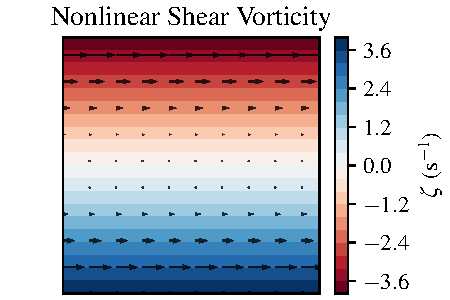
\includegraphics[width=\linewidth]{papers/rossby/images/vorticity_plot2.pdf}\\
		{\small \( \vec{u} = (y^2,0),\ \zeta = -2y\)}
	\end{minipage}
	\\[15pt]
	% Zweite Reihe
	\begin{minipage}{0.32\linewidth}
		\centering
		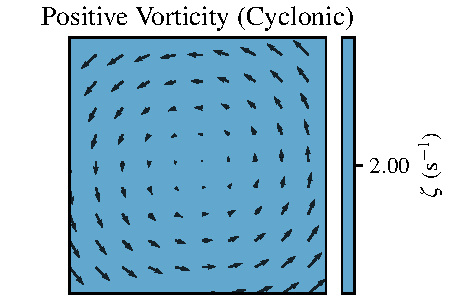
\includegraphics[width=\linewidth]{papers/rossby/images/vorticity_plot3.pdf}\\
		{\small \( \vec{u} = (-y,x),\ \zeta = 2\)}
	\end{minipage}
	\begin{minipage}{0.32\linewidth}
		\centering
		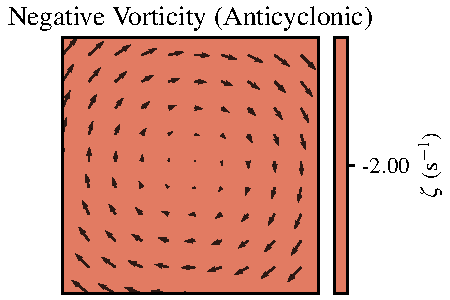
\includegraphics[width=\linewidth]{papers/rossby/images/vorticity_plot4.pdf}\\
		{\small \( \vec{u} = (y,-x),\ \zeta = -2\)}
	\end{minipage}

	\caption{Beispiele für verschiedene Vorticity-Fälle in idealisierten Strömungsfeldern.}
	\label{fig:vorticity_examples}
\end{figure}

\subsection{Absolute Vorticity}

Die bisher betrachtete relative Vorticity beschreibt die Rotation eines
Luftpakets relativ zum Erdboden. Da sich jedoch auch die Erde selbst dreht,
muss diese planetare Rotation bei der Beschreibung der Gesamtdrehung
berücksichtigt werden. Daraus ergibt sich der Begriff der \emph{absoluten
	Vorticity}, welche die Summe aus relativer und planetarer Vorticity darstellt.
\index{Vorticity, absolut}%

Die planetare Vorticity wird durch den Coriolis-Parameter \(
f = 2 \Omega \sin \varphi \) beschrieben, wobei \( \Omega \) die
Erdrotationsrate und \( \varphi \) die geographische Breite ist. Dieser
Ausdruck ergibt sich aus der Projektion der Erdrotation auf die lokale
Vertikale. Die absolute Vorticity ergibt sich somit zu:
\begin{equation}
	\eta = \zeta + f
	\label{rossby:eq:absolute_vorticity}
\end{equation}
wobei \( \zeta \) die relative und \( f \) die planetare Vorticity ist.

% Die absolute Vorticity ist eine Erhaltungsgrösse in der reibungsfreien, barotropen Atmosphäre, wenn keine vertikalen Bewegungen stattfinden.
% Sie spielt daher eine zentrale Rolle in der dynamischen Meteorologie und bildet die Grundlage für das Konzept der \emph{potenziellen Vorticity}, welches zusätzlich die Schichtung der Atmosphäre berücksichtigt.

\subsection{Potenzielle Vorticity und ihre Erhaltung}

Die \emph{potenzielle Vorticity} erweitert das Konzept der \emph{absoluten
Vorticity} um die vertikale Struktur der Atmosphäre. In ihrer Erhaltungsform
ist sie ein zentrales Werkzeug zur Beschreibung grossskaliger Strömungen und
Wellenprozesse.

Unter vereinfachten Bedingungen, barotrope, reibungsfreie Atmosphäre mit
konstantem Luftvolumen, lautet die Definition:
\begin{equation}
	q = \frac{\zeta + f}{H},
	\label{rossby:eq:potential_vorticity}
\end{equation}
wobei \(\zeta\) die relative Vorticity, \(f\) den Coriolis-Parameter und \(H\) die effektive Schichthöhe der betrachteten Luftsäule bezeichnet.
Dieser Ausdruck berücksichtigt sowohl die horizontale Rotation als auch die vertikale Ausdehnung eines Luftpakets. 

Man kann die potentielle Vorticity als die \emph{allgemeinere Erhaltungsgröße}
verstehen, welche die Drehimpulserhaltung als Spezialfall umfasst. Während
\index{Drehimpulserhaltung}%
die Drehimpulserhaltung nur die axiale Rotation einer Luftsäule beschreibt,
fasst die potentielle Vorticity zusätzlich Effekte der vertikalen Schichtung
und der relativen Vorticity zusammen. Eine anschauliche Analogie ist die
Eiskunstläufer:in, die ihre Rotationsgeschwindigkeit ändert, wenn sie die Arme
\index{Eiskunstläuferin}%
an den Körper zieht oder ausstreckt: die Drehimpulserhaltung erzwingt eine
Anpassung der Rotationsgeschwindigkeit an das veränderte Trägheitsmoment. In der
Atmosphäre entspricht dies der Anpassung der Vorticity an Änderungen der
Schichthöhe, wie sie in Gl.~\eqref{rossby:eq:potential_vorticity} beschrieben ist.



\begin{figure}
	\centering
	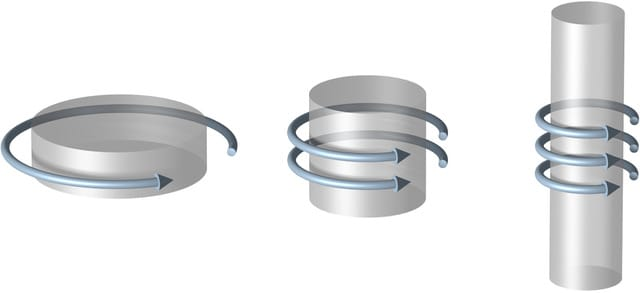
\includegraphics[width=\textwidth]{papers/rossby/images/column_streching.jpeg}


	\caption{%
		Schematische Darstellung der Erhaltung der potenziellen Vorticity.
		Die mittlere Luftsäule zeigt den Ausgangszustand mit Höhe $H$ und relativer
		Vorticity $\zeta$. Eine Verringerung der Säulenhöhe ($H \downarrow$) führt
		über horizontale Divergenz zu einer Abnahme von $|\zeta|$
		(\emph{vortex squashing}), während eine Vergrösserung ($H \uparrow$) über
		Konvergenz zu einer Zunahme von $|\zeta|$ (\emph{vortex stretching}) führt.
		Damit bleibt das Verhältnis $q=(\zeta+f)/H$ entlang der Trajektorie eines
		Luftpakets konstant (eigene Darstellung inspieriert durch \cite{rossby:beal_pv}).%
	}
	\label{fig:pv_conservation}
\end{figure}


Ein zentrales Ergebnis der quasi-geostrophischen Theorie ist die Erhaltung der
\index{quasi-geostrophisch}%
\index{Erhaltung der potenziellen Vorticity}%
potenziellen Vorticity entlang der Trajektorie eines Luftpakets:
\index{Trajektorie}%
\begin{equation}
	\frac{Dq}{Dt} = 0.
	\label{rossby:eq:pv_conservation}
\end{equation}
Unter den genannten Bedingungen treten weder Reibung noch diabatische Wärmeflüsse auf, und die Masse der Luftsäule bleibt erhalten.
\index{diabatische}%
Damit heben sich Änderungen in \(\zeta\), \(f\) und \(H\) entlang der Bewegung eines Luftpakets gegenseitig so auf, dass das Verhältnis \((\zeta + f)/H\) konstant bleibt.

Die Erhaltung der potenziellen Vorticity erklärt viele grossskalige atmosphärische Phänomene: Wird ein Luftpaket nach Norden transportiert (höheres \(f\)), so muss es zyklonale
Vorticity (\(\zeta > 0\)) abbauen oder sich ausdehnen (\(H \uparrow\)), um
\(q\) konstant zu halten. Bei einer südlichen Verlagerung gilt der umgekehrte
Mechanismus. Diese Dynamik ist eine der physikalischen Grundlagen für das
Entstehen und die Ausbreitung von Rossby-Wellen, die im folgenden Abschnitt
behandelt werden.

    \section{Rossby-Wellen}
    
% % \section{Rossby-Wellen}
% \begin{frame}{Rossby-Wellen auf der Kugel}
%     \begin{columns}
%       \column{0.55\textwidth}
%       \begin{itemize}
%         \item Idealisierte Strömung basierend auf der \textbf{Stromfunktion}:
%         \[
%           \psi(\theta, \phi) = \hat{\psi} \cos(k \phi) \sin(\theta)
%         \]
%         \item Daraus ergibt sich das Geschwindigkeitsfeld über:
%         \[
%           u = -\frac{1}{a} \frac{\partial \psi}{\partial \theta}, \quad
%           v = \frac{1}{a \sin \theta} \frac{\partial \psi}{\partial \phi}
%         \]
%         \item Wellenzahl \( k \), mittlerer Wind \( U_0 \), \\
%               Erdradius \( a \), Beta-Effekt implizit enthalten
%         \item Die Westwärts-Drift ist charakteristisch für Rossby-Wellen
%       \end{itemize}

%       \column{0.45\textwidth}
%       \centering
%       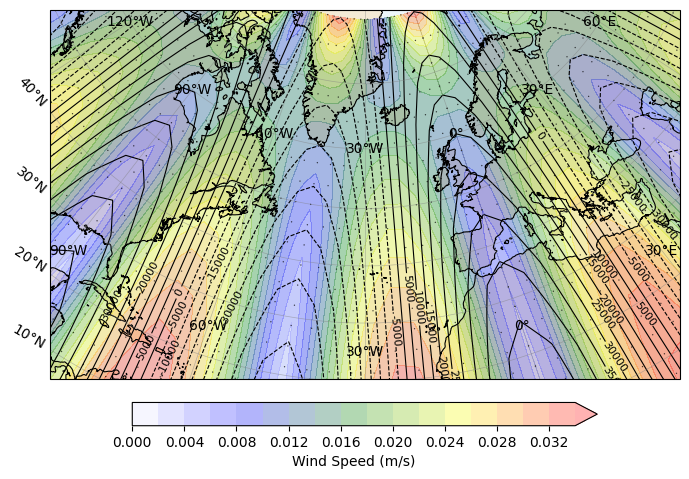
\includegraphics[width=\linewidth]{../images/rossby_wave_plot.png}
%     \end{columns}
%   \end{frame}

%   \begin{frame}{Rossby-Wellen auf der  $\beta$-Ebene}
%     \begin{columns}
%       \column{0.55\textwidth}
%       \begin{itemize}
%         \item Lineare Lösung der barotropen Vorticity-Gleichung auf der $\beta$-Ebene:
%         \[
%           \frac{\partial}{\partial t} \left( \nabla^2 \psi \right) + \beta \frac{\partial \psi}{\partial x} = 0
%         \]
%         \item Wellenansatz für die Stromfunktion:
%         \[
%           \psi(x, y, t) = \hat{\psi} \cos(kx + ly - \omega t)
%         \]
%         \item Dispersionsrelation:
%         \[
%           \omega = -\beta \frac{k}{k^2 + l^2}
%         \]
%         \item Geschwindigkeit:
%         \[
%           u = -\frac{\partial \psi}{\partial y}, \quad
%           v = \frac{\partial \psi}{\partial x}
%         \]
%         \item Charakteristisch: westwärts laufende Phasengeschwindigkeit bei \( \beta > 0 \)
%       \end{itemize}

%       \column{0.45\textwidth}
%       \centering
%       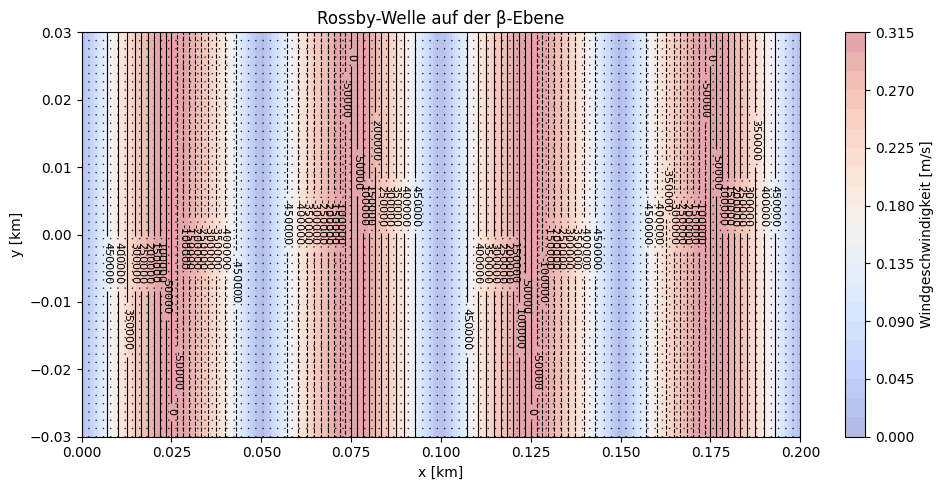
\includegraphics[width=\linewidth]{../images/rossby_wave_beta.png}
%       \scriptsize Darstellung: Windvektoren (Pfeile), Stromfunktion (schwarz), Windgeschwindigkeit (Farbflächen)
%     \end{columns}
%   \end{frame}


\begin{frame}{Mittlere Strömung und Anomalien}
	\begin{itemize}
		\item In Äquatornähe dominiert eine mittlere Ost-West-Strömung \( U \)
		\item Wir betrachten kleine Abweichungen davon:
		      \[
			      u' = U + u, \qquad v' = v \qquad \text{mit } u, v \ll U
		      \]
		\item Die Strömung ist quellenfrei → Stromfunktion \( \psi \) existiert:
		      \[
			      u = -\frac{\partial \psi}{\partial y}, \qquad v = \frac{\partial \psi}{\partial x}
		      \]
	\end{itemize}
\end{frame}

\begin{frame}{Zirkulation und Drehimpuls}
	\begin{itemize}
		\item Relative Vorticity (Zirkulation):
		      \[
			      \zeta = \frac{\partial v}{\partial x} - \frac{\partial u}{\partial y} = \Delta \psi
		      \]
		\item Absolute Vorticity:
		      \[
			      \zeta + f \qquad \text{(mit Coriolisparameter } f = f(y) \text{)}
		      \]
		\item Annahme: Erhaltung der absoluten Vorticity:
		      \[
			      \frac{d}{dt} (\zeta + f) = 0
		      \]
	\end{itemize}
\end{frame}

\begin{frame}{Bewegungsgleichung – Herleitung}
	\begin{itemize}
		\item Kettenregel für totale Ableitung:
		      \[
			      \frac{d}{dt} (\zeta + f)
			      =
			      \frac{\partial \zeta}{\partial t}
			      + (U+u) \frac{\partial \zeta}{\partial x}
			      + v \left( \frac{\partial \zeta}{\partial y} + \frac{\partial f}{\partial y} \right)
		      \]
		\item Näherungen:
		      \begin{itemize}
			      \item \( u \ll U \) → vernachlässigbar
			      \item \( \partial \zeta / \partial y \ll \partial f / \partial y \)
			      \item \( \partial f / \partial y = \beta \)
			      \item \( v = \frac{\partial \psi}{\partial x} \)
		      \end{itemize}
		\item Daraus ergibt sich:
		      \[
			      \frac{\partial \zeta}{\partial t}
			      + U \frac{\partial \zeta}{\partial x}
			      + \beta \frac{\partial \psi}{\partial x} = 0
		      \]
		\item Mit \( \zeta = \Delta \psi \):
		      \[
			      \frac{\partial \Delta \psi}{\partial t}
			      + U \frac{\partial \Delta \psi}{\partial x}
			      + \beta \frac{\partial \psi}{\partial x} = 0
		      \]
	\end{itemize}
\end{frame}

\begin{frame}{Wellenlösung der Gleichung}
	\begin{itemize}
		\item Ansatz: ebene Wellen
		      \[
			      \psi(x, y, t) = \cos(kx + ly - \omega t)
		      \]
		\item Einsetzen in Gleichung ergibt Dispersionsrelation:
		      \[
			      \omega = Uk - \frac{\beta k}{k^2 + l^2}
		      \]
		\item Phasengeschwindigkeit:
		      \[
			      c = \frac{\omega}{k} = U - \frac{\beta}{k^2 + l^2}
		      \]
		\item Interpretation: westwärts laufende Wellen mit geringer Geschwindigkeit als \( U \)
	\end{itemize}
\end{frame}

\begin{frame}{Physikalisches Feld am Beispiel der Vorticity}
  \begin{itemize}
      \item Die \textbf{Vorticity} \( \zeta(x, y, t) \) beschreibt die Rotation eines Luftpakets.
      
      \item Sie ist ein \textbf{physikalisches Skalarfeld}, das jedem Punkt eine Wirbelstärke zuordnet:
      \[
          \zeta = \frac{\partial v}{\partial x} - \frac{\partial u}{\partial y}
      \]
      
      \item In der Atmosphäre entsteht Vorticity durch:
      \begin{itemize}
          \item Wind-Scherung (Änderung der Windrichtung oder -geschwindigkeit)
          \item Bewegung entlang der Breitenkreise (\( \beta \)-Effekt)
      \end{itemize}
      
      \item Die \textbf{Vorticity-Gleichung} beschreibt, wie sich dieses Feld entwickelt:
      \[
          \frac{\partial \zeta}{\partial t} + \vec{v} \cdot \nabla \zeta + \beta v = 0
      \]
      
      \item → Diese Gleichung ist eine typische \textbf{Feldgleichung}, weil sie die Änderung eines Feldes durch lokale und advektive Prozesse beschreibt.
  \end{itemize}
  \end{frame}
  


	\section{Fazit}

	Von den grundlegenden Kräften in einem rotierenden Bezugssystem über das Konzept der relativen und potenziellen Vorticity bis hin zur Dynamik von Rossby-Wellen spannt sich ein klarer Bogen:
	Die Corioliskraft und die Erhaltung der potenziellen Vorticity liefern die physikalische Grundlage, um grossräumige atmosphärische Strömungen zu verstehen.
	Rossby-Wellen sind ein direktes Resultat dieser Prinzipien und prägen massgeblich die Wetter- und Klimadynamik der mittleren Breiten.

	Ihre Fähigkeit, über Tage bis Wochen stabile Muster zu bilden, macht sie zu einem zentralen Faktor für die Entwicklung von Hoch- und Tiefdruckgebieten - und damit auch für das Auftreten von Extremereignissen, wie das Beispiel des Sommers 2010 eindrücklich zeigt.
	Ein vertieftes Verständnis dieser Prozesse ist nicht nur für die Wettervorhersage, sondern auch für die Einschätzung künftiger Klimarisiken von Bedeutung.


	\printbibliography[heading=subbibliography]
\end{refsection}
